% Created by tikzDevice version 0.6.2-92-0ad2792 on 2013-03-04 15:04:40
% !TEX encoding = UTF-8 Unicode
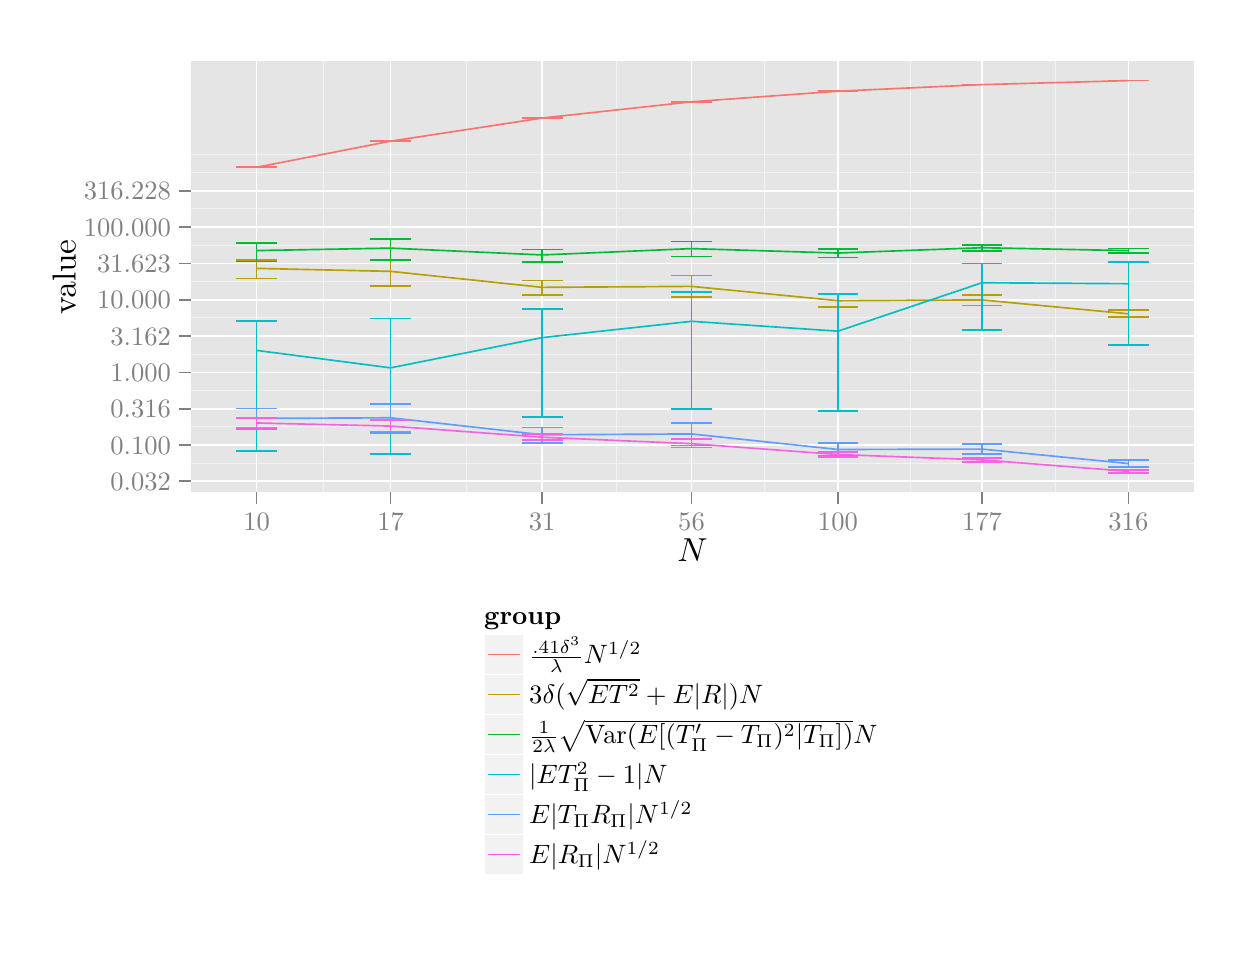
\begin{tikzpicture}[x=1pt,y=1pt]
\definecolor[named]{fillColor}{rgb}{1.00,1.00,1.00}
\path[use as bounding box,fill=fillColor,fill opacity=0.00] (0,0) rectangle (433.62,325.21);
\begin{scope}
\path[clip] (  0.00,  0.00) rectangle (433.62,325.21);
\definecolor[named]{drawColor}{rgb}{1.00,1.00,1.00}
\definecolor[named]{fillColor}{rgb}{1.00,1.00,1.00}

\path[draw=drawColor,line width= 0.6pt,line join=round,line cap=round,fill=fillColor] (  0.00,  0.00) rectangle (433.62,325.21);
\end{scope}
\begin{scope}
\path[clip] ( 58.88,157.27) rectangle (421.57,313.17);
\definecolor[named]{fillColor}{rgb}{0.90,0.90,0.90}

\path[fill=fillColor] ( 58.88,157.27) rectangle (421.57,313.17);
\definecolor[named]{drawColor}{rgb}{0.95,0.95,0.95}

\path[draw=drawColor,line width= 0.3pt,line join=round] ( 58.88,167.91) --
	(421.57,167.91);

\path[draw=drawColor,line width= 0.3pt,line join=round] ( 58.88,180.97) --
	(421.57,180.97);

\path[draw=drawColor,line width= 0.3pt,line join=round] ( 58.88,194.09) --
	(421.57,194.09);

\path[draw=drawColor,line width= 0.3pt,line join=round] ( 58.88,207.22) --
	(421.57,207.22);

\path[draw=drawColor,line width= 0.3pt,line join=round] ( 58.88,220.35) --
	(421.57,220.35);

\path[draw=drawColor,line width= 0.3pt,line join=round] ( 58.88,233.47) --
	(421.57,233.47);

\path[draw=drawColor,line width= 0.3pt,line join=round] ( 58.88,246.60) --
	(421.57,246.60);

\path[draw=drawColor,line width= 0.3pt,line join=round] ( 58.88,259.73) --
	(421.57,259.73);

\path[draw=drawColor,line width= 0.3pt,line join=round] ( 58.88,272.78) --
	(421.57,272.78);

\path[draw=drawColor,line width= 0.3pt,line join=round] ( 58.88,279.28) --
	(421.57,279.28);

\path[draw=drawColor,line width= 0.3pt,line join=round] (106.92,157.27) --
	(106.92,313.17);

\path[draw=drawColor,line width= 0.3pt,line join=round] (158.53,157.27) --
	(158.53,313.17);

\path[draw=drawColor,line width= 0.3pt,line join=round] (212.91,157.27) --
	(212.91,313.17);

\path[draw=drawColor,line width= 0.3pt,line join=round] (266.33,157.27) --
	(266.33,313.17);

\path[draw=drawColor,line width= 0.3pt,line join=round] (318.82,157.27) --
	(318.82,313.17);

\path[draw=drawColor,line width= 0.3pt,line join=round] (371.30,157.27) --
	(371.30,313.17);
\definecolor[named]{drawColor}{rgb}{1.00,1.00,1.00}

\path[draw=drawColor,line width= 0.6pt,line join=round] ( 58.88,161.42) --
	(421.57,161.42);

\path[draw=drawColor,line width= 0.6pt,line join=round] ( 58.88,174.41) --
	(421.57,174.41);

\path[draw=drawColor,line width= 0.6pt,line join=round] ( 58.88,187.52) --
	(421.57,187.52);

\path[draw=drawColor,line width= 0.6pt,line join=round] ( 58.88,200.66) --
	(421.57,200.66);

\path[draw=drawColor,line width= 0.6pt,line join=round] ( 58.88,213.78) --
	(421.57,213.78);

\path[draw=drawColor,line width= 0.6pt,line join=round] ( 58.88,226.91) --
	(421.57,226.91);

\path[draw=drawColor,line width= 0.6pt,line join=round] ( 58.88,240.04) --
	(421.57,240.04);

\path[draw=drawColor,line width= 0.6pt,line join=round] ( 58.88,253.16) --
	(421.57,253.16);

\path[draw=drawColor,line width= 0.6pt,line join=round] ( 58.88,266.29) --
	(421.57,266.29);

\path[draw=drawColor,line width= 0.6pt,line join=round] ( 82.72,157.27) --
	( 82.72,313.17);

\path[draw=drawColor,line width= 0.6pt,line join=round] (131.13,157.27) --
	(131.13,313.17);

\path[draw=drawColor,line width= 0.6pt,line join=round] (185.93,157.27) --
	(185.93,313.17);

\path[draw=drawColor,line width= 0.6pt,line join=round] (239.88,157.27) --
	(239.88,313.17);

\path[draw=drawColor,line width= 0.6pt,line join=round] (292.78,157.27) --
	(292.78,313.17);

\path[draw=drawColor,line width= 0.6pt,line join=round] (344.86,157.27) --
	(344.86,313.17);

\path[draw=drawColor,line width= 0.6pt,line join=round] (397.74,157.27) --
	(397.74,313.17);
\definecolor[named]{drawColor}{rgb}{0.97,0.46,0.43}

\path[draw=drawColor,line width= 0.6pt,line join=round] ( 82.72,274.76) --
	(131.13,284.19) --
	(185.93,292.55) --
	(239.88,298.42) --
	(292.78,302.25) --
	(344.86,304.62) --
	(397.74,306.08);
\definecolor[named]{drawColor}{rgb}{0.72,0.62,0.00}

\path[draw=drawColor,line width= 0.6pt,line join=round] ( 82.72,238.22) --
	(131.13,237.15) --
	(185.93,231.37) --
	(239.88,231.73) --
	(292.78,226.55) --
	(344.86,226.83) --
	(397.74,221.81);
\definecolor[named]{drawColor}{rgb}{0.00,0.73,0.22}

\path[draw=drawColor,line width= 0.6pt,line join=round] ( 82.72,244.66) --
	(131.13,245.54) --
	(185.93,243.08) --
	(239.88,245.37) --
	(292.78,243.77) --
	(344.86,245.69) --
	(397.74,244.64);
\definecolor[named]{drawColor}{rgb}{0.00,0.75,0.77}

\path[draw=drawColor,line width= 0.6pt,line join=round] ( 82.72,208.59) --
	(131.13,202.29) --
	(185.93,213.21) --
	(239.88,219.10) --
	(292.78,215.53) --
	(344.86,233.04) --
	(397.74,232.69);
\definecolor[named]{drawColor}{rgb}{0.38,0.61,1.00}

\path[draw=drawColor,line width= 0.6pt,line join=round] ( 82.72,184.01) --
	(131.13,184.24) --
	(185.93,178.10) --
	(239.88,178.40) --
	(292.78,172.78) --
	(344.86,172.93) --
	(397.74,167.70);
\definecolor[named]{drawColor}{rgb}{0.96,0.39,0.89}

\path[draw=drawColor,line width= 0.6pt,line join=round] ( 82.72,182.37) --
	(131.13,181.24) --
	(185.93,177.21) --
	(239.88,174.88) --
	(292.78,170.97) --
	(344.86,169.03) --
	(397.74,164.88);
\definecolor[named]{drawColor}{rgb}{0.97,0.46,0.43}

\path[draw=drawColor,line width= 0.6pt,line join=round] ( 75.37,274.76) --
	( 90.07,274.76);

\path[draw=drawColor,line width= 0.6pt,line join=round] ( 82.72,274.76) --
	( 82.72,274.76);

\path[draw=drawColor,line width= 0.6pt,line join=round] ( 75.37,274.76) --
	( 90.07,274.76);

\path[draw=drawColor,line width= 0.6pt,line join=round] (123.78,284.19) --
	(138.48,284.19);

\path[draw=drawColor,line width= 0.6pt,line join=round] (131.13,284.19) --
	(131.13,284.19);

\path[draw=drawColor,line width= 0.6pt,line join=round] (123.78,284.19) --
	(138.48,284.19);

\path[draw=drawColor,line width= 0.6pt,line join=round] (178.58,292.55) --
	(193.28,292.55);

\path[draw=drawColor,line width= 0.6pt,line join=round] (185.93,292.55) --
	(185.93,292.55);

\path[draw=drawColor,line width= 0.6pt,line join=round] (178.58,292.55) --
	(193.28,292.55);

\path[draw=drawColor,line width= 0.6pt,line join=round] (232.53,298.42) --
	(247.23,298.42);

\path[draw=drawColor,line width= 0.6pt,line join=round] (239.88,298.42) --
	(239.88,298.42);

\path[draw=drawColor,line width= 0.6pt,line join=round] (232.53,298.42) --
	(247.23,298.42);

\path[draw=drawColor,line width= 0.6pt,line join=round] (285.42,302.25) --
	(300.13,302.25);

\path[draw=drawColor,line width= 0.6pt,line join=round] (292.78,302.25) --
	(292.78,302.25);

\path[draw=drawColor,line width= 0.6pt,line join=round] (285.42,302.25) --
	(300.13,302.25);

\path[draw=drawColor,line width= 0.6pt,line join=round] (337.51,304.62) --
	(352.22,304.62);

\path[draw=drawColor,line width= 0.6pt,line join=round] (344.86,304.62) --
	(344.86,304.62);

\path[draw=drawColor,line width= 0.6pt,line join=round] (337.51,304.62) --
	(352.22,304.62);

\path[draw=drawColor,line width= 0.6pt,line join=round] (390.39,306.08) --
	(405.09,306.08);

\path[draw=drawColor,line width= 0.6pt,line join=round] (397.74,306.08) --
	(397.74,306.08);

\path[draw=drawColor,line width= 0.6pt,line join=round] (390.39,306.08) --
	(405.09,306.08);
\definecolor[named]{drawColor}{rgb}{0.72,0.62,0.00}

\path[draw=drawColor,line width= 0.6pt,line join=round] ( 75.37,241.31) --
	( 90.07,241.31);

\path[draw=drawColor,line width= 0.6pt,line join=round] ( 82.72,241.31) --
	( 82.72,234.58);

\path[draw=drawColor,line width= 0.6pt,line join=round] ( 75.37,234.58) --
	( 90.07,234.58);

\path[draw=drawColor,line width= 0.6pt,line join=round] (123.78,241.29) --
	(138.48,241.29);

\path[draw=drawColor,line width= 0.6pt,line join=round] (131.13,241.29) --
	(131.13,231.84);

\path[draw=drawColor,line width= 0.6pt,line join=round] (123.78,231.84) --
	(138.48,231.84);

\path[draw=drawColor,line width= 0.6pt,line join=round] (178.58,233.88) --
	(193.28,233.88);

\path[draw=drawColor,line width= 0.6pt,line join=round] (185.93,233.88) --
	(185.93,228.59);

\path[draw=drawColor,line width= 0.6pt,line join=round] (178.58,228.59) --
	(193.28,228.59);

\path[draw=drawColor,line width= 0.6pt,line join=round] (232.53,235.64) --
	(247.23,235.64);

\path[draw=drawColor,line width= 0.6pt,line join=round] (239.88,235.64) --
	(239.88,227.89);

\path[draw=drawColor,line width= 0.6pt,line join=round] (232.53,227.89) --
	(247.23,227.89);

\path[draw=drawColor,line width= 0.6pt,line join=round] (285.42,229.07) --
	(300.13,229.07);

\path[draw=drawColor,line width= 0.6pt,line join=round] (292.78,229.07) --
	(292.78,224.17);

\path[draw=drawColor,line width= 0.6pt,line join=round] (285.42,224.17) --
	(300.13,224.17);

\path[draw=drawColor,line width= 0.6pt,line join=round] (337.51,228.70) --
	(352.22,228.70);

\path[draw=drawColor,line width= 0.6pt,line join=round] (344.86,228.70) --
	(344.86,224.87);

\path[draw=drawColor,line width= 0.6pt,line join=round] (337.51,224.87) --
	(352.22,224.87);

\path[draw=drawColor,line width= 0.6pt,line join=round] (390.39,223.08) --
	(405.09,223.08);

\path[draw=drawColor,line width= 0.6pt,line join=round] (397.74,223.08) --
	(397.74,220.56);

\path[draw=drawColor,line width= 0.6pt,line join=round] (390.39,220.56) --
	(405.09,220.56);
\definecolor[named]{drawColor}{rgb}{0.00,0.73,0.22}

\path[draw=drawColor,line width= 0.6pt,line join=round] ( 75.37,247.48) --
	( 90.07,247.48);

\path[draw=drawColor,line width= 0.6pt,line join=round] ( 82.72,247.48) --
	( 82.72,240.75);

\path[draw=drawColor,line width= 0.6pt,line join=round] ( 75.37,240.75) --
	( 90.07,240.75);

\path[draw=drawColor,line width= 0.6pt,line join=round] (123.78,248.91) --
	(138.48,248.91);

\path[draw=drawColor,line width= 0.6pt,line join=round] (131.13,248.91) --
	(131.13,241.20);

\path[draw=drawColor,line width= 0.6pt,line join=round] (123.78,241.20) --
	(138.48,241.20);

\path[draw=drawColor,line width= 0.6pt,line join=round] (178.58,245.05) --
	(193.28,245.05);

\path[draw=drawColor,line width= 0.6pt,line join=round] (185.93,245.05) --
	(185.93,240.51);

\path[draw=drawColor,line width= 0.6pt,line join=round] (178.58,240.51) --
	(193.28,240.51);

\path[draw=drawColor,line width= 0.6pt,line join=round] (232.53,247.96) --
	(247.23,247.96);

\path[draw=drawColor,line width= 0.6pt,line join=round] (239.88,247.96) --
	(239.88,242.57);

\path[draw=drawColor,line width= 0.6pt,line join=round] (232.53,242.57) --
	(247.23,242.57);

\path[draw=drawColor,line width= 0.6pt,line join=round] (285.42,245.14) --
	(300.13,245.14);

\path[draw=drawColor,line width= 0.6pt,line join=round] (292.78,245.14) --
	(292.78,242.21);

\path[draw=drawColor,line width= 0.6pt,line join=round] (285.42,242.21) --
	(300.13,242.21);

\path[draw=drawColor,line width= 0.6pt,line join=round] (337.51,246.64) --
	(352.22,246.64);

\path[draw=drawColor,line width= 0.6pt,line join=round] (344.86,246.64) --
	(344.86,244.60);

\path[draw=drawColor,line width= 0.6pt,line join=round] (337.51,244.60) --
	(352.22,244.60);

\path[draw=drawColor,line width= 0.6pt,line join=round] (390.39,245.35) --
	(405.09,245.35);

\path[draw=drawColor,line width= 0.6pt,line join=round] (397.74,245.35) --
	(397.74,243.87);

\path[draw=drawColor,line width= 0.6pt,line join=round] (390.39,243.87) --
	(405.09,243.87);
\definecolor[named]{drawColor}{rgb}{0.00,0.75,0.77}

\path[draw=drawColor,line width= 0.6pt,line join=round] ( 75.37,219.33) --
	( 90.07,219.33);

\path[draw=drawColor,line width= 0.6pt,line join=round] ( 82.72,219.33) --
	( 82.72,172.17);

\path[draw=drawColor,line width= 0.6pt,line join=round] ( 75.37,172.17) --
	( 90.07,172.17);

\path[draw=drawColor,line width= 0.6pt,line join=round] (123.78,220.12) --
	(138.48,220.12);

\path[draw=drawColor,line width= 0.6pt,line join=round] (131.13,220.12) --
	(131.13,171.14);

\path[draw=drawColor,line width= 0.6pt,line join=round] (123.78,171.14) --
	(138.48,171.14);

\path[draw=drawColor,line width= 0.6pt,line join=round] (178.58,223.50) --
	(193.28,223.50);

\path[draw=drawColor,line width= 0.6pt,line join=round] (185.93,223.50) --
	(185.93,184.53);

\path[draw=drawColor,line width= 0.6pt,line join=round] (178.58,184.53) --
	(193.28,184.53);

\path[draw=drawColor,line width= 0.6pt,line join=round] (232.53,229.67) --
	(247.23,229.67);

\path[draw=drawColor,line width= 0.6pt,line join=round] (239.88,229.67) --
	(239.88,187.32);

\path[draw=drawColor,line width= 0.6pt,line join=round] (232.53,187.32) --
	(247.23,187.32);

\path[draw=drawColor,line width= 0.6pt,line join=round] (285.42,229.05) --
	(300.13,229.05);

\path[draw=drawColor,line width= 0.6pt,line join=round] (292.78,229.05) --
	(292.78,186.77);

\path[draw=drawColor,line width= 0.6pt,line join=round] (285.42,186.77) --
	(300.13,186.77);

\path[draw=drawColor,line width= 0.6pt,line join=round] (337.51,239.99) --
	(352.22,239.99);

\path[draw=drawColor,line width= 0.6pt,line join=round] (344.86,239.99) --
	(344.86,215.99);

\path[draw=drawColor,line width= 0.6pt,line join=round] (337.51,215.99) --
	(352.22,215.99);

\path[draw=drawColor,line width= 0.6pt,line join=round] (390.39,240.57) --
	(405.09,240.57);

\path[draw=drawColor,line width= 0.6pt,line join=round] (397.74,240.57) --
	(397.74,210.56);

\path[draw=drawColor,line width= 0.6pt,line join=round] (390.39,210.56) --
	(405.09,210.56);
\definecolor[named]{drawColor}{rgb}{0.38,0.61,1.00}

\path[draw=drawColor,line width= 0.6pt,line join=round] ( 75.37,187.61) --
	( 90.07,187.61);

\path[draw=drawColor,line width= 0.6pt,line join=round] ( 82.72,187.61) --
	( 82.72,180.05);

\path[draw=drawColor,line width= 0.6pt,line join=round] ( 75.37,180.05) --
	( 90.07,180.05);

\path[draw=drawColor,line width= 0.6pt,line join=round] (123.78,189.29) --
	(138.48,189.29);

\path[draw=drawColor,line width= 0.6pt,line join=round] (131.13,189.29) --
	(131.13,178.85);

\path[draw=drawColor,line width= 0.6pt,line join=round] (123.78,178.85) --
	(138.48,178.85);

\path[draw=drawColor,line width= 0.6pt,line join=round] (178.58,180.74) --
	(193.28,180.74);

\path[draw=drawColor,line width= 0.6pt,line join=round] (185.93,180.74) --
	(185.93,175.24);

\path[draw=drawColor,line width= 0.6pt,line join=round] (178.58,175.24) --
	(193.28,175.24);

\path[draw=drawColor,line width= 0.6pt,line join=round] (232.53,182.45) --
	(247.23,182.45);

\path[draw=drawColor,line width= 0.6pt,line join=round] (239.88,182.45) --
	(239.88,174.21);

\path[draw=drawColor,line width= 0.6pt,line join=round] (232.53,174.21) --
	(247.23,174.21);

\path[draw=drawColor,line width= 0.6pt,line join=round] (285.42,175.08) --
	(300.13,175.08);

\path[draw=drawColor,line width= 0.6pt,line join=round] (292.78,175.08) --
	(292.78,170.41);

\path[draw=drawColor,line width= 0.6pt,line join=round] (285.42,170.41) --
	(300.13,170.41);

\path[draw=drawColor,line width= 0.6pt,line join=round] (337.51,174.76) --
	(352.22,174.76);

\path[draw=drawColor,line width= 0.6pt,line join=round] (344.86,174.76) --
	(344.86,171.10);

\path[draw=drawColor,line width= 0.6pt,line join=round] (337.51,171.10) --
	(352.22,171.10);

\path[draw=drawColor,line width= 0.6pt,line join=round] (390.39,169.01) --
	(405.09,169.01);

\path[draw=drawColor,line width= 0.6pt,line join=round] (397.74,169.01) --
	(397.74,166.45);

\path[draw=drawColor,line width= 0.6pt,line join=round] (390.39,166.45) --
	(405.09,166.45);
\definecolor[named]{drawColor}{rgb}{0.96,0.39,0.89}

\path[draw=drawColor,line width= 0.6pt,line join=round] ( 75.37,184.09) --
	( 90.07,184.09);

\path[draw=drawColor,line width= 0.6pt,line join=round] ( 82.72,184.09) --
	( 82.72,180.56);

\path[draw=drawColor,line width= 0.6pt,line join=round] ( 75.37,180.56) --
	( 90.07,180.56);

\path[draw=drawColor,line width= 0.6pt,line join=round] (123.78,183.46) --
	(138.48,183.46);

\path[draw=drawColor,line width= 0.6pt,line join=round] (131.13,183.46) --
	(131.13,179.29);

\path[draw=drawColor,line width= 0.6pt,line join=round] (123.78,179.29) --
	(138.48,179.29);

\path[draw=drawColor,line width= 0.6pt,line join=round] (178.58,178.37) --
	(193.28,178.37);

\path[draw=drawColor,line width= 0.6pt,line join=round] (185.93,178.37) --
	(185.93,176.11);

\path[draw=drawColor,line width= 0.6pt,line join=round] (178.58,176.11) --
	(193.28,176.11);

\path[draw=drawColor,line width= 0.6pt,line join=round] (232.53,176.50) --
	(247.23,176.50);

\path[draw=drawColor,line width= 0.6pt,line join=round] (239.88,176.50) --
	(239.88,173.46);

\path[draw=drawColor,line width= 0.6pt,line join=round] (232.53,173.46) --
	(247.23,173.46);

\path[draw=drawColor,line width= 0.6pt,line join=round] (285.42,171.97) --
	(300.13,171.97);

\path[draw=drawColor,line width= 0.6pt,line join=round] (292.78,171.97) --
	(292.78,170.12);

\path[draw=drawColor,line width= 0.6pt,line join=round] (285.42,170.12) --
	(300.13,170.12);

\path[draw=drawColor,line width= 0.6pt,line join=round] (337.51,169.79) --
	(352.22,169.79);

\path[draw=drawColor,line width= 0.6pt,line join=round] (344.86,169.79) --
	(344.86,168.22);

\path[draw=drawColor,line width= 0.6pt,line join=round] (337.51,168.22) --
	(352.22,168.22);

\path[draw=drawColor,line width= 0.6pt,line join=round] (390.39,165.41) --
	(405.09,165.41);

\path[draw=drawColor,line width= 0.6pt,line join=round] (397.74,165.41) --
	(397.74,164.35);

\path[draw=drawColor,line width= 0.6pt,line join=round] (390.39,164.35) --
	(405.09,164.35);
\end{scope}
\begin{scope}
\path[clip] (  0.00,  0.00) rectangle (433.62,325.21);
\definecolor[named]{drawColor}{rgb}{0.50,0.50,0.50}

\node[text=drawColor,anchor=base east,inner sep=0pt, outer sep=0pt, scale=  0.96] at ( 51.77,158.11) {0.032};

\node[text=drawColor,anchor=base east,inner sep=0pt, outer sep=0pt, scale=  0.96] at ( 51.77,171.10) {0.100};

\node[text=drawColor,anchor=base east,inner sep=0pt, outer sep=0pt, scale=  0.96] at ( 51.77,184.22) {0.316};

\node[text=drawColor,anchor=base east,inner sep=0pt, outer sep=0pt, scale=  0.96] at ( 51.77,197.35) {1.000};

\node[text=drawColor,anchor=base east,inner sep=0pt, outer sep=0pt, scale=  0.96] at ( 51.77,210.48) {3.162};

\node[text=drawColor,anchor=base east,inner sep=0pt, outer sep=0pt, scale=  0.96] at ( 51.77,223.60) {10.000};

\node[text=drawColor,anchor=base east,inner sep=0pt, outer sep=0pt, scale=  0.96] at ( 51.77,236.73) {31.623};

\node[text=drawColor,anchor=base east,inner sep=0pt, outer sep=0pt, scale=  0.96] at ( 51.77,249.86) {100.000};

\node[text=drawColor,anchor=base east,inner sep=0pt, outer sep=0pt, scale=  0.96] at ( 51.77,262.98) {316.228};
\end{scope}
\begin{scope}
\path[clip] (  0.00,  0.00) rectangle (433.62,325.21);
\definecolor[named]{drawColor}{rgb}{0.50,0.50,0.50}

\path[draw=drawColor,line width= 0.6pt,line join=round] ( 54.61,161.42) --
	( 58.88,161.42);

\path[draw=drawColor,line width= 0.6pt,line join=round] ( 54.61,174.41) --
	( 58.88,174.41);

\path[draw=drawColor,line width= 0.6pt,line join=round] ( 54.61,187.52) --
	( 58.88,187.52);

\path[draw=drawColor,line width= 0.6pt,line join=round] ( 54.61,200.66) --
	( 58.88,200.66);

\path[draw=drawColor,line width= 0.6pt,line join=round] ( 54.61,213.78) --
	( 58.88,213.78);

\path[draw=drawColor,line width= 0.6pt,line join=round] ( 54.61,226.91) --
	( 58.88,226.91);

\path[draw=drawColor,line width= 0.6pt,line join=round] ( 54.61,240.04) --
	( 58.88,240.04);

\path[draw=drawColor,line width= 0.6pt,line join=round] ( 54.61,253.16) --
	( 58.88,253.16);

\path[draw=drawColor,line width= 0.6pt,line join=round] ( 54.61,266.29) --
	( 58.88,266.29);
\end{scope}
\begin{scope}
\path[clip] (  0.00,  0.00) rectangle (433.62,325.21);
\definecolor[named]{drawColor}{rgb}{0.50,0.50,0.50}

\path[draw=drawColor,line width= 0.6pt,line join=round] ( 82.72,153.00) --
	( 82.72,157.27);

\path[draw=drawColor,line width= 0.6pt,line join=round] (131.13,153.00) --
	(131.13,157.27);

\path[draw=drawColor,line width= 0.6pt,line join=round] (185.93,153.00) --
	(185.93,157.27);

\path[draw=drawColor,line width= 0.6pt,line join=round] (239.88,153.00) --
	(239.88,157.27);

\path[draw=drawColor,line width= 0.6pt,line join=round] (292.78,153.00) --
	(292.78,157.27);

\path[draw=drawColor,line width= 0.6pt,line join=round] (344.86,153.00) --
	(344.86,157.27);

\path[draw=drawColor,line width= 0.6pt,line join=round] (397.74,153.00) --
	(397.74,157.27);
\end{scope}
\begin{scope}
\path[clip] (  0.00,  0.00) rectangle (433.62,325.21);
\definecolor[named]{drawColor}{rgb}{0.50,0.50,0.50}

\node[text=drawColor,anchor=base,inner sep=0pt, outer sep=0pt, scale=  0.96] at ( 82.72,143.54) {10};

\node[text=drawColor,anchor=base,inner sep=0pt, outer sep=0pt, scale=  0.96] at (131.13,143.54) {17};

\node[text=drawColor,anchor=base,inner sep=0pt, outer sep=0pt, scale=  0.96] at (185.93,143.54) {31};

\node[text=drawColor,anchor=base,inner sep=0pt, outer sep=0pt, scale=  0.96] at (239.88,143.54) {56};

\node[text=drawColor,anchor=base,inner sep=0pt, outer sep=0pt, scale=  0.96] at (292.78,143.54) {100};

\node[text=drawColor,anchor=base,inner sep=0pt, outer sep=0pt, scale=  0.96] at (344.86,143.54) {177};

\node[text=drawColor,anchor=base,inner sep=0pt, outer sep=0pt, scale=  0.96] at (397.74,143.54) {316};
\end{scope}
\begin{scope}
\path[clip] (  0.00,  0.00) rectangle (433.62,325.21);
\definecolor[named]{drawColor}{rgb}{0.00,0.00,0.00}

\node[text=drawColor,anchor=base,inner sep=0pt, outer sep=0pt, scale=  1.20] at (240.23,132.27) {$N$};
\end{scope}
\begin{scope}
\path[clip] (  0.00,  0.00) rectangle (433.62,325.21);
\definecolor[named]{drawColor}{rgb}{0.00,0.00,0.00}

\node[text=drawColor,rotate= 90.00,anchor=base,inner sep=0pt, outer sep=0pt, scale=  1.20] at ( 17.30,235.22) {value};
\end{scope}
\begin{scope}
\path[clip] (  0.00,  0.00) rectangle (433.62,325.21);
\definecolor[named]{fillColor}{rgb}{1.00,1.00,1.00}

\path[fill=fillColor] (160.71, 14.89) rectangle (319.75,120.39);
\end{scope}
\begin{scope}
\path[clip] (  0.00,  0.00) rectangle (433.62,325.21);
\definecolor[named]{drawColor}{rgb}{0.00,0.00,0.00}

\node[text=drawColor,anchor=base west,inner sep=0pt, outer sep=0pt, scale=  0.96] at (164.98,109.50) {\bfseries group};
\end{scope}
\begin{scope}
\path[clip] (  0.00,  0.00) rectangle (433.62,325.21);
\definecolor[named]{drawColor}{rgb}{1.00,1.00,1.00}
\definecolor[named]{fillColor}{rgb}{0.95,0.95,0.95}

\path[draw=drawColor,line width= 0.6pt,line join=round,line cap=round,fill=fillColor] (164.98, 91.43) rectangle (179.43,105.88);
\end{scope}
\begin{scope}
\path[clip] (  0.00,  0.00) rectangle (433.62,325.21);
\definecolor[named]{drawColor}{rgb}{0.97,0.46,0.43}

\path[draw=drawColor,line width= 0.6pt,line join=round] (166.42, 98.66) -- (177.98, 98.66);
\end{scope}
\begin{scope}
\path[clip] (  0.00,  0.00) rectangle (433.62,325.21);
\definecolor[named]{drawColor}{rgb}{0.97,0.46,0.43}

\path[draw=drawColor,line width= 0.6pt,line join=round] (166.42, 98.66) -- (177.98, 98.66);
\end{scope}
\begin{scope}
\path[clip] (  0.00,  0.00) rectangle (433.62,325.21);
\definecolor[named]{drawColor}{rgb}{1.00,1.00,1.00}
\definecolor[named]{fillColor}{rgb}{0.95,0.95,0.95}

\path[draw=drawColor,line width= 0.6pt,line join=round,line cap=round,fill=fillColor] (164.98, 76.97) rectangle (179.43, 91.43);
\end{scope}
\begin{scope}
\path[clip] (  0.00,  0.00) rectangle (433.62,325.21);
\definecolor[named]{drawColor}{rgb}{0.72,0.62,0.00}

\path[draw=drawColor,line width= 0.6pt,line join=round] (166.42, 84.20) -- (177.98, 84.20);
\end{scope}
\begin{scope}
\path[clip] (  0.00,  0.00) rectangle (433.62,325.21);
\definecolor[named]{drawColor}{rgb}{0.72,0.62,0.00}

\path[draw=drawColor,line width= 0.6pt,line join=round] (166.42, 84.20) -- (177.98, 84.20);
\end{scope}
\begin{scope}
\path[clip] (  0.00,  0.00) rectangle (433.62,325.21);
\definecolor[named]{drawColor}{rgb}{1.00,1.00,1.00}
\definecolor[named]{fillColor}{rgb}{0.95,0.95,0.95}

\path[draw=drawColor,line width= 0.6pt,line join=round,line cap=round,fill=fillColor] (164.98, 62.52) rectangle (179.43, 76.97);
\end{scope}
\begin{scope}
\path[clip] (  0.00,  0.00) rectangle (433.62,325.21);
\definecolor[named]{drawColor}{rgb}{0.00,0.73,0.22}

\path[draw=drawColor,line width= 0.6pt,line join=round] (166.42, 69.75) -- (177.98, 69.75);
\end{scope}
\begin{scope}
\path[clip] (  0.00,  0.00) rectangle (433.62,325.21);
\definecolor[named]{drawColor}{rgb}{0.00,0.73,0.22}

\path[draw=drawColor,line width= 0.6pt,line join=round] (166.42, 69.75) -- (177.98, 69.75);
\end{scope}
\begin{scope}
\path[clip] (  0.00,  0.00) rectangle (433.62,325.21);
\definecolor[named]{drawColor}{rgb}{1.00,1.00,1.00}
\definecolor[named]{fillColor}{rgb}{0.95,0.95,0.95}

\path[draw=drawColor,line width= 0.6pt,line join=round,line cap=round,fill=fillColor] (164.98, 48.07) rectangle (179.43, 62.52);
\end{scope}
\begin{scope}
\path[clip] (  0.00,  0.00) rectangle (433.62,325.21);
\definecolor[named]{drawColor}{rgb}{0.00,0.75,0.77}

\path[draw=drawColor,line width= 0.6pt,line join=round] (166.42, 55.29) -- (177.98, 55.29);
\end{scope}
\begin{scope}
\path[clip] (  0.00,  0.00) rectangle (433.62,325.21);
\definecolor[named]{drawColor}{rgb}{0.00,0.75,0.77}

\path[draw=drawColor,line width= 0.6pt,line join=round] (166.42, 55.29) -- (177.98, 55.29);
\end{scope}
\begin{scope}
\path[clip] (  0.00,  0.00) rectangle (433.62,325.21);
\definecolor[named]{drawColor}{rgb}{1.00,1.00,1.00}
\definecolor[named]{fillColor}{rgb}{0.95,0.95,0.95}

\path[draw=drawColor,line width= 0.6pt,line join=round,line cap=round,fill=fillColor] (164.98, 33.61) rectangle (179.43, 48.07);
\end{scope}
\begin{scope}
\path[clip] (  0.00,  0.00) rectangle (433.62,325.21);
\definecolor[named]{drawColor}{rgb}{0.38,0.61,1.00}

\path[draw=drawColor,line width= 0.6pt,line join=round] (166.42, 40.84) -- (177.98, 40.84);
\end{scope}
\begin{scope}
\path[clip] (  0.00,  0.00) rectangle (433.62,325.21);
\definecolor[named]{drawColor}{rgb}{0.38,0.61,1.00}

\path[draw=drawColor,line width= 0.6pt,line join=round] (166.42, 40.84) -- (177.98, 40.84);
\end{scope}
\begin{scope}
\path[clip] (  0.00,  0.00) rectangle (433.62,325.21);
\definecolor[named]{drawColor}{rgb}{1.00,1.00,1.00}
\definecolor[named]{fillColor}{rgb}{0.95,0.95,0.95}

\path[draw=drawColor,line width= 0.6pt,line join=round,line cap=round,fill=fillColor] (164.98, 19.16) rectangle (179.43, 33.61);
\end{scope}
\begin{scope}
\path[clip] (  0.00,  0.00) rectangle (433.62,325.21);
\definecolor[named]{drawColor}{rgb}{0.96,0.39,0.89}

\path[draw=drawColor,line width= 0.6pt,line join=round] (166.42, 26.39) -- (177.98, 26.39);
\end{scope}
\begin{scope}
\path[clip] (  0.00,  0.00) rectangle (433.62,325.21);
\definecolor[named]{drawColor}{rgb}{0.96,0.39,0.89}

\path[draw=drawColor,line width= 0.6pt,line join=round] (166.42, 26.39) -- (177.98, 26.39);
\end{scope}
\begin{scope}
\path[clip] (  0.00,  0.00) rectangle (433.62,325.21);
\definecolor[named]{drawColor}{rgb}{0.00,0.00,0.00}

\node[text=drawColor,anchor=base west,inner sep=0pt, outer sep=0pt, scale=  0.96] at (181.24, 95.35) {$\frac{.41\delta^3}{\lambda}N^{1/2}\quad $};
\end{scope}
\begin{scope}
\path[clip] (  0.00,  0.00) rectangle (433.62,325.21);
\definecolor[named]{drawColor}{rgb}{0.00,0.00,0.00}

\node[text=drawColor,anchor=base west,inner sep=0pt, outer sep=0pt, scale=  0.96] at (181.24, 80.90) {$3\delta(\sqrt{\mathbb{E}T^2}+\mathbb{E}|R|)N\quad $};
\end{scope}
\begin{scope}
\path[clip] (  0.00,  0.00) rectangle (433.62,325.21);
\definecolor[named]{drawColor}{rgb}{0.00,0.00,0.00}

\node[text=drawColor,anchor=base west,inner sep=0pt, outer sep=0pt, scale=  0.96] at (181.24, 66.44) {$\frac{1}{2\lambda}\sqrt{\mathrm{Var}(\mathbb{E}[(T'_{\Pi}-T_{\Pi})^2|T_{\Pi}])}N\quad $};
\end{scope}
\begin{scope}
\path[clip] (  0.00,  0.00) rectangle (433.62,325.21);
\definecolor[named]{drawColor}{rgb}{0.00,0.00,0.00}

\node[text=drawColor,anchor=base west,inner sep=0pt, outer sep=0pt, scale=  0.96] at (181.24, 51.99) {$|\mathbb{E}T_{\Pi}^2-1|N\quad $};
\end{scope}
\begin{scope}
\path[clip] (  0.00,  0.00) rectangle (433.62,325.21);
\definecolor[named]{drawColor}{rgb}{0.00,0.00,0.00}

\node[text=drawColor,anchor=base west,inner sep=0pt, outer sep=0pt, scale=  0.96] at (181.24, 37.53) {$\mathbb{E}|T_{\Pi}R_{\Pi}|N^{1/2}\quad $};
\end{scope}
\begin{scope}
\path[clip] (  0.00,  0.00) rectangle (433.62,325.21);
\definecolor[named]{drawColor}{rgb}{0.00,0.00,0.00}

\node[text=drawColor,anchor=base west,inner sep=0pt, outer sep=0pt, scale=  0.96] at (181.24, 23.08) {$\mathbb{E}|R_{\Pi}|N^{1/2}\quad $};
\end{scope}
\end{tikzpicture}
